% =============================================================================
% Slide deck 2 -- ambient-electron exchange thruster, EP-engineer audience
% Build: pdflatex slides2.tex (twice).
% Structure: concept -> data -> physics -> mission -> honesty.
% New figures in figs2/; shared assets in ../figs/.
% =============================================================================
\documentclass[10pt,aspectratio=169]{beamer}
\usetheme{default}
\usecolortheme{seahorse}
\setbeamertemplate{navigation symbols}{}
\setbeamertemplate{footline}[frame number]
\setbeamercolor{frametitle}{fg=blue!30!black}
\setbeamerfont{frametitle}{series=\bfseries,size=\large}
\usepackage{booktabs,tikz,graphicx}
\graphicspath{{figs2/}{../figs/}}
\newcommand{\srcnote}[1]{\vfill{\tiny\color{gray}#1}}

\title{Propellantless Drag Compensation by Ambient-Electron Exchange}
\subtitle{Measured PIC frontier \quad pre-registered predictions \quad
zero propellant}
\author{R.~S.~C.}
\date{August 2026}

\begin{document}

% 1 --- Title -----------------------------------------------------------------
\begin{frame}
  \titlepage
\end{frame}

% 2 --- The gap ---------------------------------------------------------------
\begin{frame}{Drag is nanonewtons --- no flight thruster reaches that low}
  \centering
  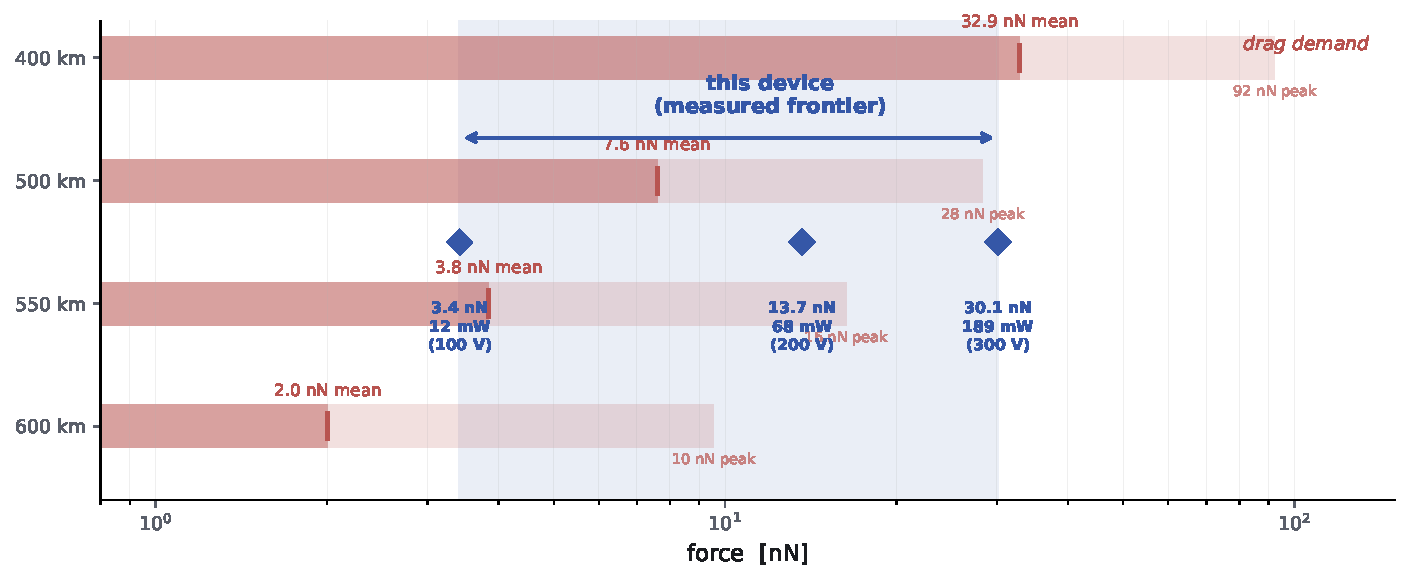
\includegraphics[width=0.95\linewidth]{demand_supply.pdf}
  \begin{itemize}\small
    \item LEO drag at 500--600\,km: \textbf{2--8\,nN mean} for a
          kg-class CubeSat.
    \item Smallest flight EP (FEEP/electrospray): 5--30\,\textmu N,
          $\ge$8\,W --- $10^2$--$10^3\times$ above the demand.
    \item Dry-system floor (tank + feed + valves + PPU) $\approx$ 0.3--1\,kg:
          a large share of a kilogram-class CubeSat.
  \end{itemize}
\end{frame}

% 3 --- Concept ---------------------------------------------------------------
\begin{frame}{You already fly this device --- as a neutralizer}
  \begin{columns}
    \column{0.48\textwidth}
      \centering
      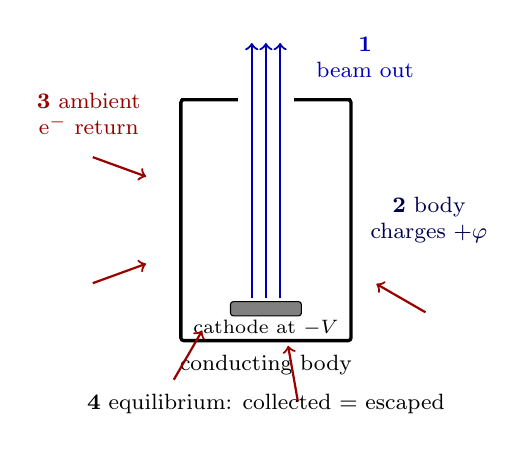
\begin{tikzpicture}[scale=0.9, every node/.style={font=\small}]
        % body
        \draw[very thick, rounded corners=1pt] (0,0) rectangle (2.4,3.4);
        % aperture gap
        \draw[very thick,white,line width=4pt] (0.8,3.4) -- (1.6,3.4);
        \draw[very thick] (0,3.4) -- (0.8,3.4);
        \draw[very thick] (1.6,3.4) -- (2.4,3.4);
        \node[font=\footnotesize] at (1.2,-0.35) {conducting body};
        % cathode
        \draw[fill=black!50, rounded corners=1pt] (0.7,0.35) rectangle (1.7,0.55);
        \node[font=\scriptsize] at (1.2,0.18) {cathode at $-V$};
        % beam arrows
        \foreach \x in {1.0,1.2,1.4}
          \draw[->,thick,blue!70!black] (\x,0.6) -- (\x,4.2);
        \node[blue!70!black,font=\footnotesize,align=center] at (2.6,4.0)
          {\textbf{1}\\beam out};
        % body charges
        \node[font=\footnotesize,blue!30!black,align=center] at (3.5,1.7)
          {\textbf{2} body\\charges $+\varphi$};
        % returning electrons
        \foreach \a in {160,200,240,280,330}
          \draw[<-,thick,red!60!black]
            ({1.2+1.8*cos(\a)},{1.7+1.8*sin(\a)}) --
            ({1.2+2.6*cos(\a)},{1.7+2.6*sin(\a)});
        \node[red!60!black,font=\footnotesize,align=center] at (-1.3,3.2)
          {\textbf{3} ambient\\e$^-$ return};
        % equilibrium
        \node[font=\footnotesize,align=center] at (1.2,-0.9)
          {\textbf{4} equilibrium: collected = escaped};
      \end{tikzpicture}
    \column{0.50\textwidth}
      {\small
      \begin{enumerate}
        \item Supply holds cathode at $-V$; electrons accelerate out
              through the aperture.
        \item Body charges positive ($+\varphi$).
        \item Ionosphere returns electrons to the skin until
              $I_{\mathrm{collected}} = I_{\mathrm{escaped}}$.
        \item \textbf{The ionosphere is both propellant tank and
              neutralizer.}
      \end{enumerate}}
      \vspace{1ex}
      \begin{itemize}
        \item[\textbullet] \small\textbf{Hardware:} an HV supply, a cold gun, a hole.
        \item[\textbullet] \small Every ion/Hall thruster already carries the gun ---
              run it alone and it \emph{is} this thruster.
      \end{itemize}
  \end{columns}
\end{frame}

% 4 --- Momentum cancellation -------------------------------------------------
\begin{frame}{``The current comes back --- doesn't the momentum cancel?''}
  \begin{columns}
    \column{0.52\textwidth}
      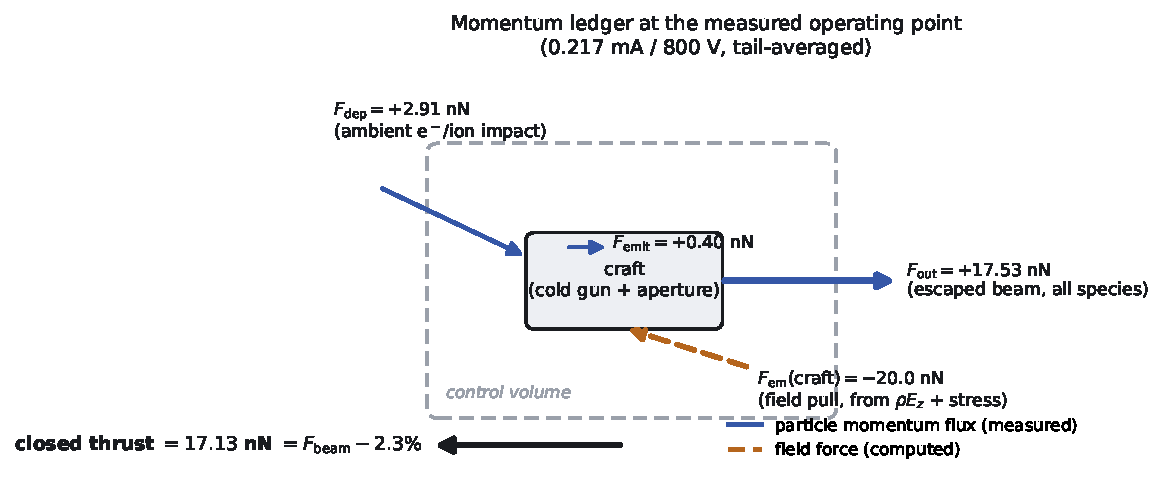
\includegraphics[width=\linewidth]{ledger_diagram.pdf}
    \column{0.46\textwidth}
      \textbf{Full-return null test:} body pinned above beam energy,
      escape $= 0$\%.\\[0.5ex]
      \small Impact channel: $-12.1$\,nN.\\
      Closed thrust: $-0.39$\,nN $\approx 0$. \hfill $\checkmark$\\[1.5ex]
      \normalsize\textbf{At the operating points:}\\[0.5ex]
      \small Return-channel momentum vs beam thrust:\\
      \textbf{1.0\%} at 300\,V \quad (0.30 vs 30.1\,nN)\\
      \textbf{8.8\%} at 100\,V\\[1.5ex]
      \normalsize\textbf{Physics ceiling:} collected e$^-$ arrive
      isotropically at $\sim e\varphi$ vs directed exhaust at
      $\sim$210\,eV --- even fully anti-directed arrival cancels
      $\le$41\%.
  \end{columns}
\end{frame}

% 5 --- Measured frontier ------------------------------------------------------
\begin{frame}{The frontier is measured, not projected}
  \centering
  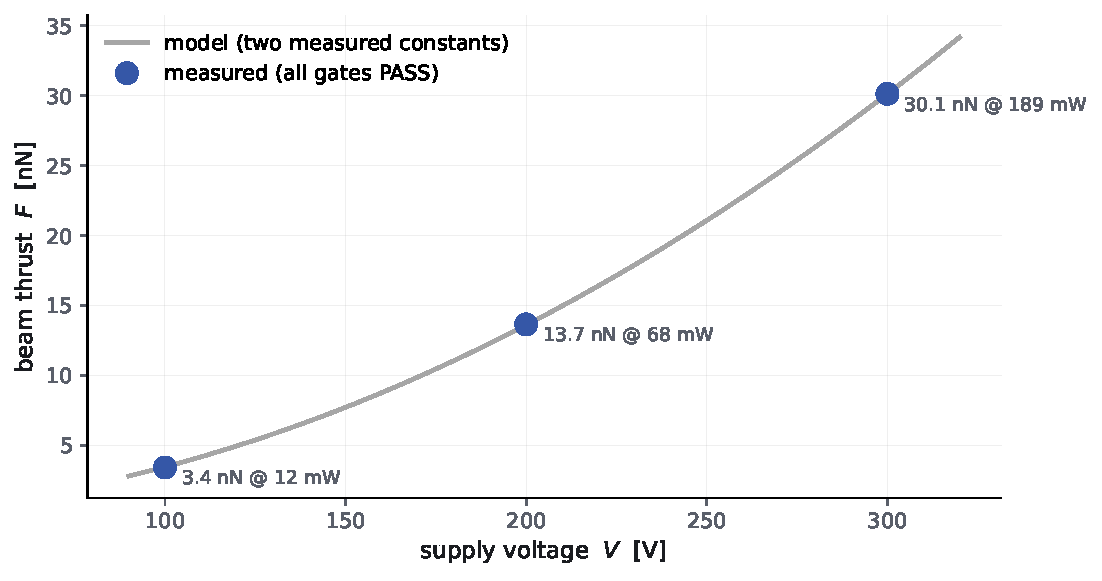
\includegraphics[width=0.85\linewidth]{frontier_thrust.pdf}
  \vspace{0.5ex}
  \begin{itemize}\small
    \item Three production runs across the full 100--300\,V hardware
          range; \textbf{all pre-registered acceptance gates PASS}.
    \item Thrust landed $<$1\,\% from predictions recorded in the
          repository before the runs completed.
  \end{itemize}
\end{frame}

% 6 --- Collection law ---------------------------------------------------------
\begin{frame}{The collection law was decided by experiment}
  \begin{columns}
    \column{0.55\textwidth}
      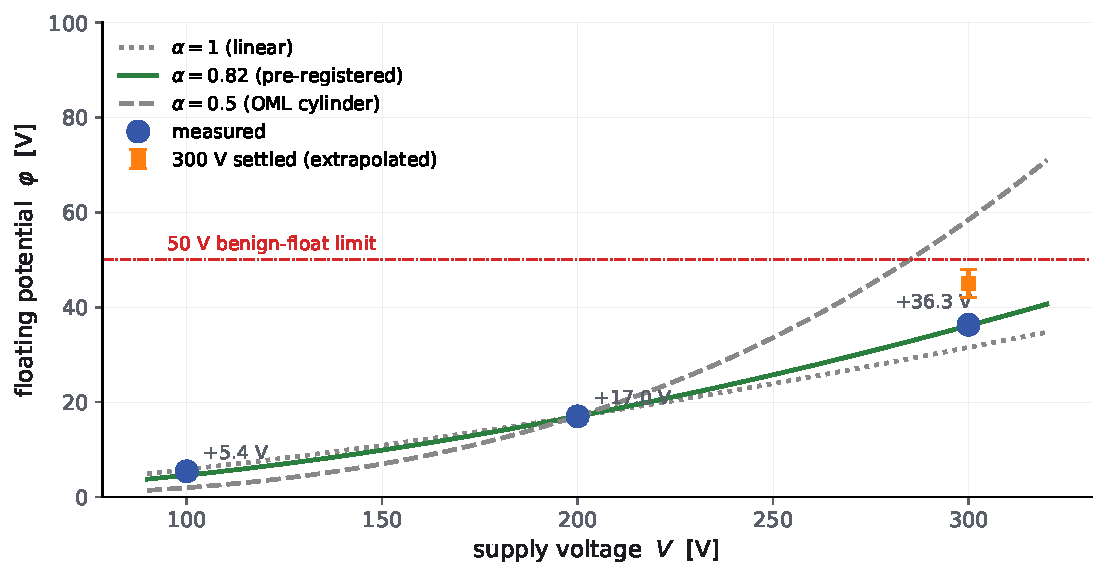
\includegraphics[width=\linewidth]{frontier_phi.pdf}
    \column{0.43\textwidth}
      \small Collected current:
      $I = \beta A\, j_{\mathrm{the}}\,(1+\chi)^{\alpha}$,
      \ $\chi = e\varphi/kT_e$.\\[1ex]
      Three exponents, all agreeing at 200\,V, diverging at 300\,V.
      Predictions recorded before the run:
      \vspace{0.5ex}
      \begin{center}\footnotesize
      \begin{tabular}{lcc}
        \toprule
        law & predicted $\varphi$ & verdict \\
        \midrule
        $\alpha = 1$ & 31\,V & \textcolor{red}{refuted} \\
        $\alpha = 0.82$ & 36\,V & \textcolor{green!50!black}{\textbf{survives}} \\
        $\alpha = 0.5$ & 90\,V & \textcolor{red}{refuted} \\
        \midrule
        \textbf{measured} & \textbf{36.3\,V} \\
        \bottomrule
      \end{tabular}
      \end{center}
      \vspace{0.5ex}
      \small Fit across all three points: $\alpha = 0.85$--0.89.\\
      Closes the analytical power model to 4--6\%.
  \end{columns}
\end{frame}

% 7 --- F/P by design ---------------------------------------------------------
\begin{frame}{$F/P$ is 200$\times$ below your Hall thruster --- by design}
  \begin{columns}[T]
    \column{0.46\textwidth}
      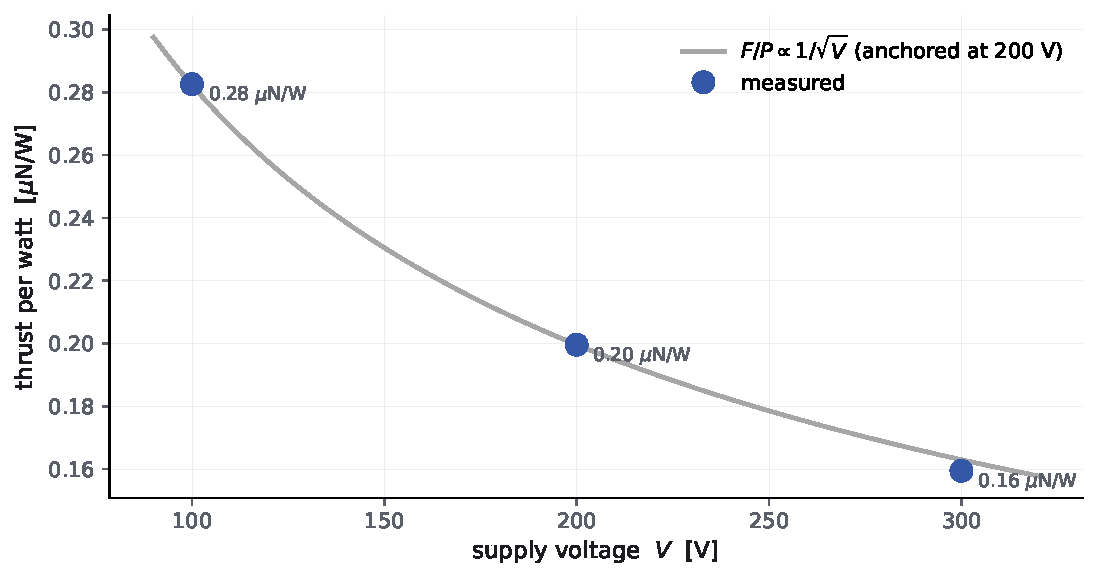
\includegraphics[width=\linewidth]{frontier_fp.pdf}
    \column{0.46\textwidth}
      \centering\small
      \begin{tabular}{lccc}
        \toprule
         & \textbf{this work} & electrospray & Hall \\
        \midrule
        $\eta_{\mathrm{jet}}$ & \textbf{68--73\,\%} & 28--45\,\% & 31--44\,\% \\
        $F/P$ [\textmu N/W] & 0.16--0.28 & $\sim$5 & $\sim$50 \\
        \bottomrule
      \end{tabular}
      \vspace{1.5ex}

      \raggedright
      Both rows are true at once \emph{because the exhaust is
      electrons}: superb energy-to-jet conversion at tiny momentum
      per watt.\\[1ex]
      The $F/P$ penalty is \textbf{invisible at nN}, noticeable at
      \textmu N, decisive at mN.\\[1ex]
      \textbf{Below $\sim$0.1\,\textmu N}: us.\\
      \textbf{\textmu N}: electrospray.\\
      \textbf{mN}: ion/Hall.\\[0.5ex]
      Complement, not competitor.
  \end{columns}
\end{frame}

% 8 --- Density axis -----------------------------------------------------------
\begin{frame}{Density axis: the law is conservative}
  \begin{columns}
    \column{0.50\textwidth}
      \small The $n_e/3$ continuation (2.4\,\textmu s) is the
      campaign's only \textbf{fully settled float}:
      \begin{itemize}\small
        \item Pre-registered predictions:
              $\alpha{=}1$: 53\,V;\
              0.82: 68\,V;\
              0.5: 160\,V.
        \item \textbf{Measured: $+42.5$\,V, settled}
              ($-0.14$\,V/\textmu s, flat to noise).
        \item $\alpha = 0.5$ refuted a second time.
        \item Every fixed exponent \emph{overshoots}
              $\Rightarrow$ the fitted law is \textbf{conservative
              along density}.
      \end{itemize}
    \column{0.48\textwidth}
      \small Thin plasma does \emph{not} end the envelope:
      \begin{itemize}\small
        \item 42.5\,V clears the 50\,V benign limit (a run
              this axis was expected to break).
        \item $F = 12.39$\,nN; escape 99.1\,\%;
              KE 122.0 vs 122.6\,eV predicted.
        \item All acceptance gates PASS.
      \end{itemize}
      \vspace{1ex}
      \centering\footnotesize
      \begin{tabular}{lcc}
        \toprule
        & anchor ($n_0$) & thin ($n_0/3$) \\
        \midrule
        $\varphi$ [V] & $+17.0$ & $+42.5$ \\
        escape & 98.4\,\% & 99.1\,\% \\
        settled? & no (800\,ns) & \textbf{yes} (2.4\,\textmu s) \\
        \bottomrule
      \end{tabular}
  \end{columns}
\end{frame}

% 9 --- B field ----------------------------------------------------------------
\begin{frame}{Geomagnetic field: operating point untouched at flight strength}
  \begin{columns}
    \column{0.50\textwidth}
      \small\textbf{30\,\textmu T (flight strength):}
      \begin{itemize}\small
        \item $\varphi$: 17.22 vs 16.98\,V (no field).
        \item $F$: 13.64 vs 13.65\,nN.
        \item Escape within 0.06\,pp.
        \item Pre-registered null \textbf{holds on every bound}.
        \item Beam gyroradius $\ge$0.10\,m $\gg$ device.
      \end{itemize}
    \column{0.48\textwidth}
      \small\textbf{300\,\textmu T (10$\times$, amplification):}
      \begin{itemize}\small
        \item A collection tax through the float:\\
              $\varphi = +32.6$\,V (vs $+17.0$\,V).
        \item Beam formation \emph{unaffected}:\\
              escape 98.3\,\%.
        \item The two-constant thrust law reproduces both:\\
              13.56 / 12.03\,nN predicted vs\\
              13.64 / 12.06\,nN measured.
      \end{itemize}
      \vspace{1ex}
      \small The field acts on \emph{collection} only --- not on
      beam formation.
  \end{columns}
\end{frame}

% 10 --- Size cancels ----------------------------------------------------------
\begin{frame}{Size cancels: the corridor carries to CubeSats}
  \centering
  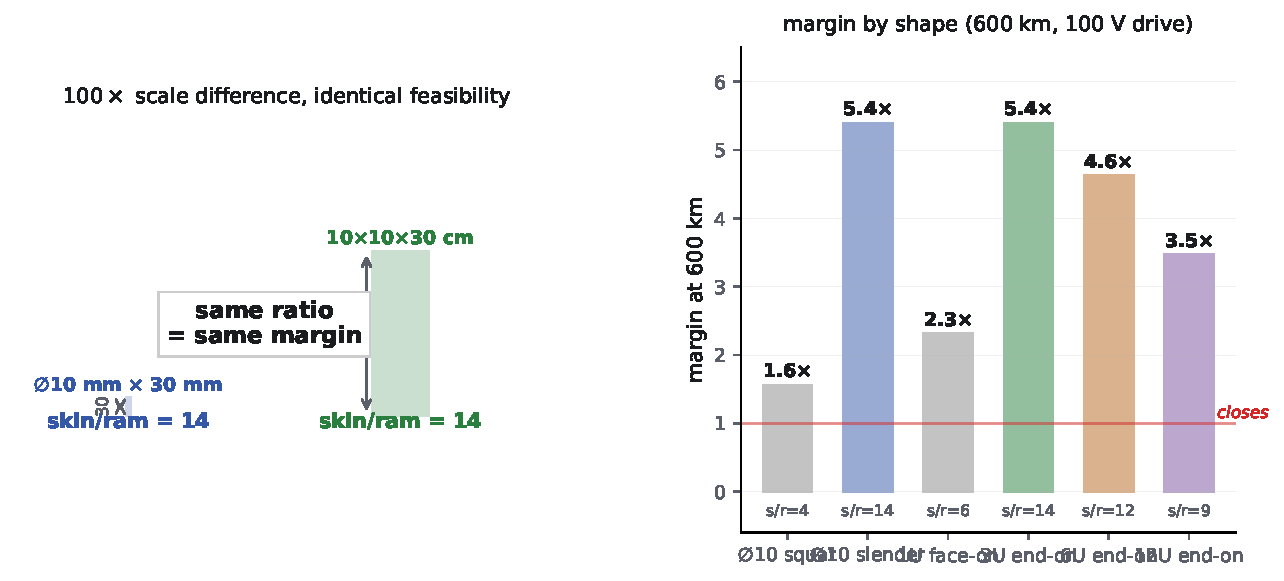
\includegraphics[width=0.90\linewidth]{scale_visual.pdf}
  \begin{itemize}\small
    \item Drag charges \textbf{ram silhouette}; collection and any
          body-mounted supply pay from \textbf{skin}. Both areal
          $\Rightarrow$ \textbf{size cancels}.
    \item 3U at 600\,km: 8.8\,mA / 0.88\,W. Bigger is
          \emph{less} extrapolated.
    \item Caveat: CubeSat radii 25--60\,$\lambda_D$ (vs 2.5
          measured) --- different sheath regime, \textbf{not yet run}.
  \end{itemize}
\end{frame}

% 11 --- Mission corridor ------------------------------------------------------
\begin{frame}{Mission corridor --- with the failures stated plainly}
  \centering
  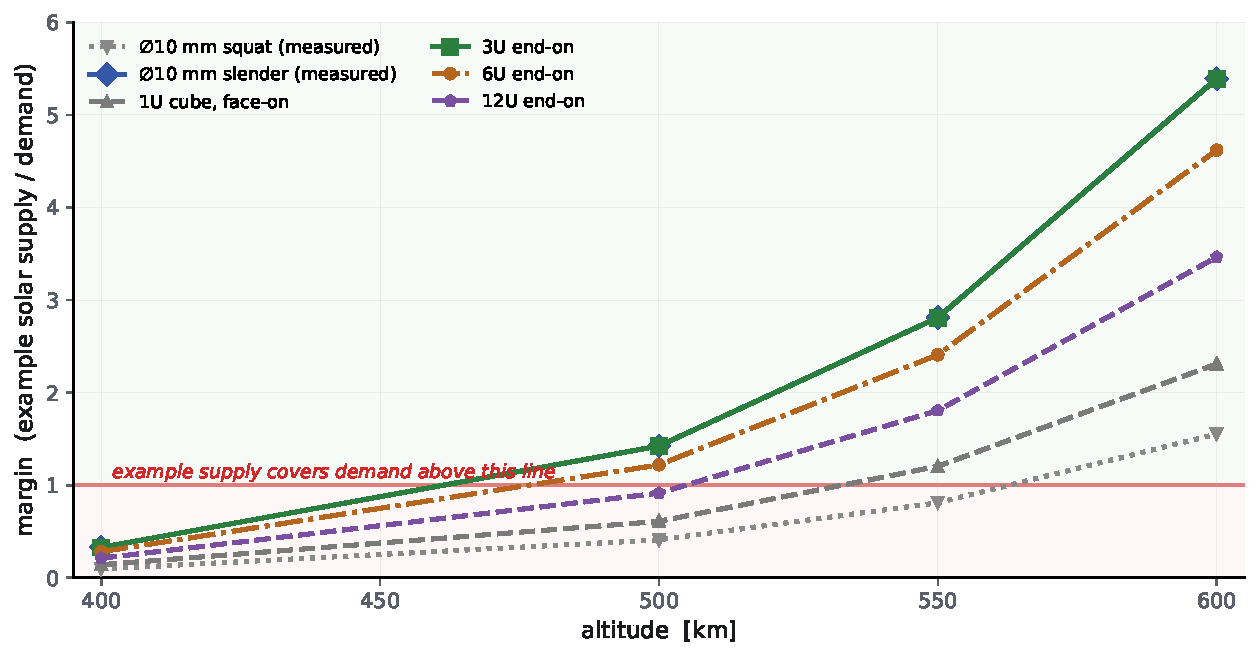
\includegraphics[width=0.80\linewidth]{margin_corridor.pdf}
  \begin{itemize}\small
    \item Year-long propagations, real F10.7/Ap, per-5-min plasma +
          drag; minimum-power $(V, I, \varphi)$ solved each step.
    \item \textbf{Closes at 550--600\,km}; impulse-closes at 500\,km;
          \textbf{does not close at 400\,km} for any shape.
    \item Slender bodies: $\varphi$ drops 17 $\to$ 4.4\,V; thrust
          \emph{rises} to 14.2\,nN at same silhouette.
  \end{itemize}
\end{frame}

% 12 --- Honest limits ---------------------------------------------------------
\begin{frame}{Where the model is still blind}
  \begin{columns}
    \column{0.50\textwidth}
      \small\textbf{Measured axes:}
      \begin{itemize}\small
        \item \textbf{Voltage}: three-point frontier, all gates
              PASS, model closes to 4--6\,\%.
        \item \textbf{Density}: one $3\times$ step (settled, law
              conservative). Deeper night rows remain extrapolation.
        \item \textbf{Geometry}: slender body to $L/r = 6$;
              beyond that, open.
        \item \textbf{$B$ field}: axial pair. Flight null holds;
              transverse far field cannot be posed in RZ ---
              \emph{open}.
      \end{itemize}
    \column{0.48\textwidth}
      \small\textbf{Known approximations:}
      \begin{itemize}\small
        \item Reduced ion mass ($400\,m_e$ vs O$^+$ 29\,166).
        \item Stationary plasma (no ram wake).
        \item RZ symmetry (no 3D effects).
        \item Powers are beam power $I\,V$; converter and cathode
              overheads not included.
      \end{itemize}
      \vspace{1ex}
      \small\textbf{Highest-value next run:}\\
      CubeSat sheath regime (25--60\,$\lambda_D$).\\
      Lower $\chi$ $\Rightarrow$ faster settle.
  \end{columns}
  \srcnote{Every row outside the measured envelope is flagged, never
  averaged in.}
\end{frame}

% 13 --- Take-away -------------------------------------------------------------
\begin{frame}{Take-away}
  \begin{enumerate}
    \item \textbf{The frontier is measured}: 3.4\,nN @ 12\,mW to
          30\,nN @ 189\,mW, all gates PASS, predictions
          pre-registered.
    \item \textbf{The thrust is real}: full-return null closes to
          zero; return-channel momentum $\le$9\,\% of beam thrust.
    \item \textbf{The collection law is discriminated on two axes}
          and is \emph{conservative} along density; the geomagnetic
          field leaves the operating point untouched at flight
          strength.
    \item \textbf{The mission corridor is honest}: closes at
          550--600\,km; fails at 400\,km and says so.
    \item \textbf{Size cancels}: a 3U CubeSat inherits the corridor
          unchanged.
  \end{enumerate}
  \vspace{2ex}
  \centering
  \large\emph{Cheap to test on orbit: it's a gun and a hole.}
\end{frame}

% ============================ BACKUPS =========================================
\appendix

\begin{frame}{Backup: spacecraft charging detail}
  \begin{columns}
    \column{0.50\textwidth}
      \begin{itemize}\small
        \item The float $\varphi$ is the state variable: it rises
              until the ionosphere returns exactly the escaped
              current.
        \item The float robs the beam: accelerating potential is
              always $V - \varphi$ (charging tax: 5\,\% at 100\,V,
              12\,\% at 300\,V).
        \item Gated benign ($\varphi \le 50$\,V) on every run; a
              choke detector aborts any run the ionosphere cannot
              neutralize.
      \end{itemize}
    \column{0.48\textwidth}
      \centering
      \begin{tabular}{lccc}
        \toprule
        $V$ [V] & 100 & 200 & 300 \\
        \midrule
        $\varphi$ [V] & $+5.4$ & $+17.0$ & $+36.3$ \\
        escape & 96.1\,\% & 98.4\,\% & 99.0\,\% \\
        balance & 1.5\,\% & 3.2\,\% & 3.5\,\% \\
        \bottomrule
      \end{tabular}
  \end{columns}
\end{frame}

\begin{frame}{Backup: the throttle principle}
  \begin{block}{Ideal law (measured constants; near-unity escape,
      $\varphi \ll V$)}
    \centering\small
    \begin{tabular}{l}
      $F = \sqrt{2m_e/e}\; I\sqrt{\mathrm{KE}}$
        \hfill (beam momentum flux)\\[0.4ex]
      $P = V I \;\Rightarrow\; P = F\sqrt{V}/c_{\mathrm{ideal}}$,\quad
        $c_{\mathrm{ideal}} = \sqrt{2m_e/e}$\\[0.4ex]
      throttle: largest feasible escaped current, lowest sufficient
        voltage\\[0.4ex]
      \footnotesize PIC: $c_F = 0.97\,c_{\mathrm{ideal}}$ (divergence),
        $\kappa = 0.81$ (space charge) $\Rightarrow$ 1.19--1.22$\times$
        the parameter-free bound\\
    \end{tabular}
  \end{block}
  \begin{itemize}\small
    \item Model: 11.7 / 65.8 / 177.9\,mW vs measured 12.1 / 68.4 /
          189\,mW --- within 4--6\,\%.
    \item Residual is the charging tax $V/(V-\varphi)$.
  \end{itemize}
\end{frame}

\begin{frame}{Backup: how we know (evidence stack)}
  \begin{columns}
    \column{0.50\textwidth}
      \small\textbf{Per run (all gated):}
      \begin{itemize}\small
        \item Frozen, hashed physics config; manifest with seed,
              code version, git commit.
        \item 7--8 acceptance gates fixed \emph{before} the run;
              zero waived.
        \item Ledger vs independent particle dumps: agreement at
              $10^{-9}$ (gate $2\times10^{-2}$).
      \end{itemize}
    \column{0.48\textwidth}
      \small\textbf{Campaign-level:}
      \begin{itemize}\small
        \item Validation ladder: thermal collection $\pm$1\,\% vs
              theory $\to$ biased $\to$ floating $\to$ gun rungs.
        \item Code-to-code parity: $\varphi$ 0.05\,\%, escape
              0.001\,\%, $F$ 0.09\,\%.
        \item PPC$\times$2 shifts $\le$0.05\,\%; grid
              ($0.15\to0.10$\,mm): $F$ $+4.0$\,\%, KE $+7.4$\,\%
              --- carried as the error band.
      \end{itemize}
  \end{columns}
\end{frame}

\begin{frame}{Backup: settle time and the 300\,V late-slope caveat}
  \begin{itemize}\small
    \item Body $\approx$ capacitor charged by the escaping beam:
          $\tau \approx C\varphi/I_{\mathrm{esc}} \approx 28$\,ns;
          every run spans $\approx$29$\tau$.
    \item At high $\chi$ the sheath equilibrates on the \emph{ion}
          timescale: the 300\,V late slope decayed $+44 \to
          +27$\,mV/ns but was nonzero at 800\,ns.
    \item Settled-value extrapolation: $\varphi_\infty \approx
          42$--48\,V --- inside the 50\,V gate.
    \item The $n_e/3$ continuation (2.4\,\textmu s) is the only
          fully settled float.
  \end{itemize}
\end{frame}

\begin{frame}{Backup: numerics detail}
  \begin{itemize}\small
    \item WarpX 26.5 (GPU), RZ electrostatic, embedded-boundary
          conductor with per-step charge-pump float update; particle
          reservoir (infinite-ionosphere recycle).
    \item Grid 0.15\,mm ($\lambda_D = 1.97$\,mm); CFL $dt$; 16 ppc;
          800\,ns per production run; $\sim$7\,h on an RTX 3060.
    \item PPC$\times$2 at the anchor: all 8 gates PASS. Grid
          $0.15\to0.10$\,mm: $F$ $+4.0$\,\%, KE $+7.4$\,\%.
    \item Reduced ion mass $400\,m_e$: ladder-wide, disclosed.
  \end{itemize}
\end{frame}

\begin{frame}{Backup: ``why not a tether?''}
  \begin{itemize}\small
    \item Conceded: per watt, electrodynamic-tether thrust at km
          scale beats any reaction engine.
    \item For the bodies here the comparison inverts:
    \begin{itemize}\small
      \item A CubeSat vs a deployed, stabilized conductor
            $10^3$--$10^6\times$ its own length.
      \item Thrust constrained to
            $I\mathbf{L}\times\mathbf{B}$ direction.
      \item A bare tether still needs electron collection and
            emission at its ends --- the same contactor physics
            this device is, minus the tether.
    \end{itemize}
    \item Related physics is our foundation, not competitor:
          bare-tether OML collection (Sanmart\'in 1993), PMG
          plasma contactors (1993), E-sail electron gun (Janhunen).
  \end{itemize}
\end{frame}

\begin{frame}{Backup: F/P plane (incumbent context)}
  \centering
  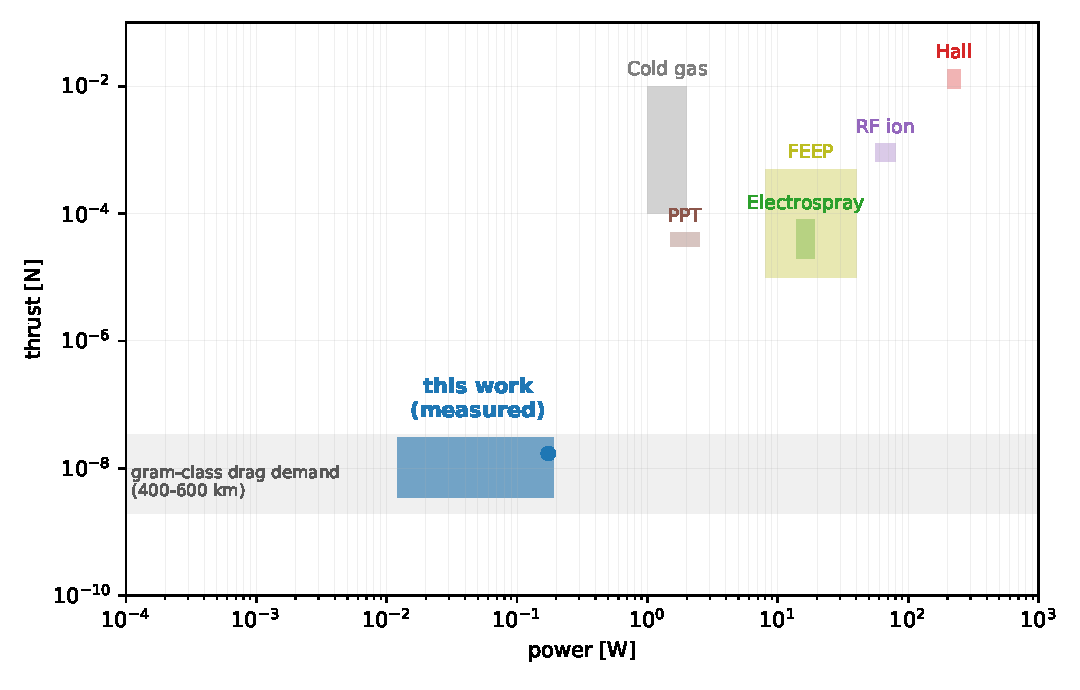
\includegraphics[width=0.75\linewidth]{fp_plane.pdf}
  \srcnote{Incumbent ranges: NASA SoA Small Spacecraft Technology 2026;
  manufacturer datasheets (see paper Table 2).}
\end{frame}

\begin{frame}{Backup: propellant accounting}
  \begin{itemize}\small
    \item ``Propellant'' = ambient electrons: $\dot m = (m_e/e)\,I
          \approx 2\times10^{-15}$\,kg/s at 0.342\,mA $\approx$
          \textbf{60\,ng/year}.
    \item Effective $I_{\mathrm{sp}} \sim 10^{6}$\,s --- not a
          merit figure (electrons are nearly free, momentum-poor
          mass); quoted only for EP bookkeeping.
    \item Five years of nN thrust $\approx$ 5\,N\,s $\approx$
          0.3\,g electrospray propellant: the argument is never
          propellant \emph{mass} --- it is the \textbf{dry-system
          floor}.
  \end{itemize}
\end{frame}

\end{document}
